\documentclass[10pt]{article}
\usepackage[top=0.5in,left=0.75in,footskip=0.5in,marginparwidth=1in]{geometry}

% use Unicode characters - try changing the option if you run into troubles with special characters (e.g. umlauts)
\usepackage[utf8]{inputenc}
\usepackage{amsmath}
\usepackage{amssymb,amsthm}
\usepackage{hyperref}
\usepackage[normalem]{ulem}
\usepackage{mathabx}
\usepackage{multicol,lipsum,graphicx,float}
% clean citations
\usepackage{cite}
\usepackage{fixltx2e}
% hyperref makes references clicky. use \url{www.example.com} or \href{www.example.com}{description} to add a clicky url
\usepackage{nameref,hyperref}

 %line numbers
\usepackage[right]{lineno}

% improves typesetting in LaTeX
\usepackage{microtype}
\DisableLigatures[f]{encoding = *, family = * }

% text layout - change as needed
%\raggedright
%\setlength{\parindent}{0.7cm}
\textwidth 7.5in 
\textheight 9.5in

% Remove % for double line spacing
%\usepackage{setspace} 
%\doublespacing

% use adjustwidth environment to exceed text width (see examples in text)
\usepackage{changepage}
\usepackage{indentfirst}

% adjust caption style
\usepackage[aboveskip=1pt,labelfont=bf,labelsep=period,singlelinecheck=off]{caption}

% remove brackets from references
\makeatletter
\renewcommand{\@biblabel}[1]{\quad#1.}
\makeatother

% headrule, footrule and page numbers
\usepackage{lastpage,fancyhdr,graphicx}
\usepackage{epstopdf}
\pagestyle{myheadings}
\pagestyle{fancy}
\fancyhf{}
\rfoot{\thepage/\pageref{LastPage}}
\renewcommand{\footrule}{\hrule height 2pt \vspace{2mm}}
\fancyheadoffset[L]{1.25in}
\fancyfootoffset[L]{2.25in}

% use \textcolor{color}{text} for colored text (e.g. highlight to-do areas)
\usepackage{color}

% define custom colors (this one is for figure captions)
\definecolor{Gray}{gray}{.25}

% this is required to include graphics
\usepackage{graphicx}

% use if you want to put caption to the side of the figure - see example in text
\usepackage{sidecap}

% use for have text wrap around figures
\usepackage{wrapfig}
\usepackage[pscoord]{eso-pic}
\usepackage[fulladjust]{marginnote}
\reversemarginpar

\usepackage{sectsty}
\sectionfont{\fontsize{12}{15}\selectfont}
\subsectionfont{\fontsize{10}{12}\selectfont}
% document begins here
\begin{document}
% title goes here:
\begin{flushleft}
{\Large
\bf{Multi-Level Monte Carlo Algorithm for Integrate-Fire Neural Network}
}
\newline
% authors go here:
\begin{center}
Zhuocheng Xiao\textsuperscript{1}, 
Kevin Lin\textsuperscript{1,*} 
\end{center} 
\begin{center}
\bf{1} Department of Mathematics, University of Arizona
\end{center}
* klin@math.arizona.edu
\end{flushleft}

\section*{Abstract}
\noindent
Multi-Level Monte Carlo algorithm is much more efficient to simulate SDEs, comparing with MC algorithm. The core idea for MLMC is using information from different levels of numerical results to constraint mean-square-error (MSE), so that we gain a better estimation on the expectation. For coarser discretization, we evolve more samples, and less samples for finer discretization. Comparing with MC, when we try to get the same order of accuracy of estimation, we could use the MSE produced by the finest grid and the largest group of samples, which has shown huge advantages on time cost. However, when we try to apply MLMC to I-F Neuron network, we need to face several questions which people didn't know the answers before, which drives us to write this work report...(need modification)

\bigskip
% now start line numbers
%\linenumbers

% the * after section prevents numbering
\begin{multicols}{2}


\section{Introduction}
\noindent
Action potentials, which are the reactions of neurons to stimulation, play a critical role in neuron interaction by transmitting signals along connected neurons in  central nervous system. %, which are also the main component for neural-network activities
Action potentials are also named as "neural spikes" or "firing events" due to the short millisecond-time-scales, comparing with the collective behavior of a group of neurons in several seconds. The "spike sequences" generated by a neural network are signals released to the network itself/other neural system, therefore usually viewed as the core study object of computational neuroscience. One can use spike sequences to describe the functions of a group of neurons, or examine relation between different brain areas, or event reconstruct a stimulus-driven network from the exact spike times. \\
\indent
As the central character of brain coding, the spike sequences should be captured by a successful numerical simulation of neural dynamics with satisfying time accuracy. A classical approximative model called Leaky-Integrate-Fire (LIF) Equations are commonly used in computation. A much simplyfied current-based LIF for a single neuron is like: 
\begin{subequations}
\begin{align}
     \frac{\mbox{d}v}{\mbox{d}t}& =  - g_L(v-V_r)+I, \label{simIF}\\
    \tau \frac{\mbox{d}I}{\mbox{d}t}&=-I+f \sum_{\mu}\delta(t-t_{\mu}) \nonumber\\
     v(t^-)=V_T &\Leftrightarrow v(t^+)= V_{r}. \label{simBC}
\end{align}
\end{subequations}
\ref{simIF} is a differential equation describing dynamics of the neuron's membrane potential and current, with jump boundary condition \ref{simBC} (reset to 0 when $v$ reach 1). Current $I$ is driven by a stochastic $\delta-$sequence $\mu$ which are the spikes received by this neuron. Therefore, such kind of LIF equations can be evolved by Monte Carlo method for large amount of samples. Monte Carlo path simulation methods are frequently employed in numerical simulations to gain statistics for a stochastic processes, especially stochastic differential equations(SDEs). However, even for the simplist stastic, expectation $\mathbb{E}(X)$, an estimation with an $O(\epsilon)$ mean-square-error brings an $O(\epsilon)^{-3}$ time cost \cite{Giles2008}. Thus, variance reduction methods are used extensively to cut down computation complexity to gain fast and accurate statistics. In 2008, M. Giles developed an multigrid method for variance reduction \cite{Giles2008}, which is called Multi-Level Monte Carlo algorithm (MLMC). Here, we are trying to apply this algorithem to evolving the dynamics of neural networks. As people are mostly using the classical Monte Carlo method (named as MC below) for the task, MLMC is capable to remarkably reduce the computational complexity from $O(\epsilon^3)$ to $O(\epsilon^2 log(\epsilon))$, according to {\bf{Theorem 3.1}} in \cite{Giles2008}.
\begin{figure}[H] %s state preferences regarding figure placement here
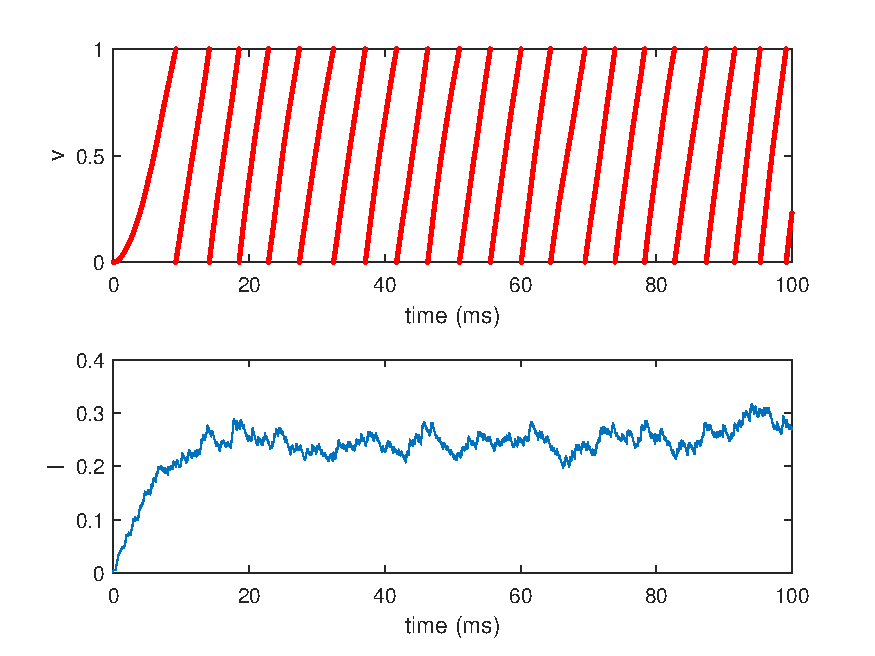
\includegraphics[width=0.5\textwidth]{VI_plots.pdf}
\caption{\color{Gray}A 100-ms numerical sample for \ref{simIF}, assuming input firing events $\mu$ to be Poission. The upper bar for $V$ and the lower bar for $I$. Driven byexcitory input firing events, $V$ keeps crossing the boundary. The numerical result for $I(t)$ is just like a Ohrnstein-Uhlenbeck process, intuitively leading us to \ref{sIF}, i.e., the current jumps $\sum_{\mu^{E}}f\delta(t-t_{\mu})$ could be approximatied by a Wiener process.}
\label{VI_plots} % \label works only AFTER \caption within figure environment
\end{figure}
\indent
To utilize numerical solutions from different grids to cancel the errors introduced by numerical grids, we need them converging to an actual solution (if exists!) when the grid size $h\rightarrow0$. This is pretty natual if the stochastic differential equations (SDE) are continuous and satisfy Lipschitz condition. In LIF equation, however, this is generally not true according to the jumping boundary condition \ref{simBC}. There are plenty of researches on SDE with jump, but none of them was about a jump boundary condition. That's to say, if an error $\epsilon$ produced at some step, the time boundness or convergence for such $\epsilon(t)$ is never guaranteed by any classical numerical approximation theorm. Without any further investigation into error estimation for LIF eqns, we can't trust the numerical solution to {\bf{a single neuron}}, not to mention MLMC method which is based on the former.\\
\indent
Such obstacle drives us to look into the convergence of numerical error for LIF equations in detail. In this article, we present a "physical proof" for almost sure convergence of membrane potential $v$ when evolved by same/different time grid sizes. Based on such convergence, we can derive convergence for every Feed-Forward Network (FFN), i.e. we can safely use MLMC methods for FFNs. As for recurrent network (neural network with feed back), however, the situation is much more complicated. We argue that for weakly coupled networks which don't produce multiple firing events (MFEs) \cite{MFE}, a.s. convergence still esists. But for strongly coupled networks with large MFEs, a.s. convergence collapses and numerical results are extremely sensitive to time error for even a single firing event. In this case, MLMC method is no more valid when simulations don't converge even if taking grid size $h\rightarrow0$.  

\section{Background}
\subsection{Simplified LIF Equations}
The membrane potential and current dynamics of  a general current-based LIF neural network consists of Excitory \& Inhibitory neurons with various connectivity can be described as:
\begin{subequations}
\begin{align}
    C\frac{\mbox{d}v_{j}}{\mbox{d}t} &=  - g_L(v_j-V_{r})+(I^{E}_{j}-I^I_{j}), \nonumber \\
    \sigma_E\frac{\mbox{d}I^{E}_{j}}{\mbox{d}t} &= -I^{E}_{j}+\sum_{\mu^{E}_{j}}f^{E}_{j}\delta(t-t_{\mu^{E}_{j}}) + \sum_{i\neq j}\sum_{\mu^{E}_{ij}}s^{E}_{ij}\delta(t-t_{\mu^{E}_{ij}}), \nonumber \\
    \sigma_I\frac{\mbox{d}I^I_{j}}{\mbox{d}t} &= -I^I_{j}+\sum_{\mu^I_{j}}f^I_{j}\delta(t-t_{\mu^I_{j}}) + \sum_{i\neq j}\sum_{\mu^I_{ij}}s^I_{ij}\delta(t-t_{\mu^I_{ij}}). \label{nIF}\\
    & v_{j}\in (-\infty, V_T),\quad  I^{E,I}_{j}\in [0,+\infty); \nonumber\\
    & v_{j}(t^-)=V_T \Leftrightarrow v_{j}(t^+)= V_{r}. \label{BC}
\end{align}
\end{subequations}
In \ref{nIF}, $\mu^{E,I}_{j}$ represent Excitory \& inhibitory input spiking sequences, which can be assumed as Poission processes in many cases. So $\mu^{E,I}_{j}$ is the source of stochasticity for the system. On the other hand, matrices $[\mu]^{E,I}_{ij}$ represent Excitory or inhibitory connections from neuron $i$ to neuron $j$.\\ 
\indent
We will start from a single neuron in {\bf Coupling Single Neurons}, as the dynamics for a neural network could be so sophisticated. Consider the I-F eqn for a single neuron:
\begin{subequations}
\begin{align}
    C\frac{\mbox{d}v}{\mbox{d}t} &=  - g_Lv+(I^{E}-I^I), \nonumber\\
    \sigma_E\frac{\mbox{d}I^{E}}{\mbox{d}t} &= -I^E+\sum_{\mu^{E}}f^{E}\delta(t-t_{\mu^{E}}),  \nonumber\\ \label{1IF}
    \sigma_I\frac{\mbox{d}I^I}{\mbox{d}t} &= -I^I+\sum_{\mu^I}f^I\delta(t-t_{\mu^I}). 
\end{align}
\end{subequations}
In \ref{1IF}, we simply choose $C = 1, V_r = 0, V_T = 1, g_L = \frac{1}{20\mbox{ms}}$ and $\sigma_E = \sigma_I = 5$ms. Furthermore, we can simply assume the inhibitory current $I^I$ is a constant for simplicity as firing dynamics is mainly determined by $I^{E}$ like the case in Fig.\ref{VI_plots}. Note that $\mu^{E}$ is supposed as Poission with frequency $\nu$ and could well-approximated by Gaussian processes when we take limit $f^E\to 0,\nu\to \infty$. Thus, we could rewrite \ref{1IF} as:
\begin{subequations}
\begin{align}
    \frac{\mbox{d}v}{\mbox{d}t} &=  - g_Lv+(I^{E}-I^I), \label{sIF1} \\ 
    \sigma_E\frac{\mbox{d}I^{E}}{\mbox{d}t} &= -I^E+f\nu+\frac{f^2\nu}{2}\frac{\mbox{d}W}{\mbox{d}t}.\label{sIF2}
\end{align}
\end{subequations}
What's more, by taking $\sigma_E\to0\Rightarrow I^E = f\nu+\frac{f^2\nu}{2}\frac{\mbox{d}W}{\mbox{d}t}$, \ref{sIF1} and \ref{sIF2} are homogenized into a 1-variable SDE with jumping boundary condition, directly driven by a white noise:
\indent
\begin{equation}
\frac{\mbox{d}v}{\mbox{d}t} =  - g_Lv+(f\nu+\frac{f^2\nu}{2}\frac{\mbox{d}W}{\mbox{d}t}-I^I). \label{sIF}
\end{equation}

\subsection{Couplings and Sensitivity}
A valid numerical simulation for a sample from \ref{sIF} requires convergent error. Consider sample $v$ and a biased sample $u=v+\epsilon(t)$ and their coupling $P(v,u)$ which is a joint probability space for them, where both samples driven by the exactly same input. Therefore, finite coupling time and $\lim_{t\to\infty}|u-v|=0$ leads to a valid numerical method. \\
\indent
For "real" solutions, as we have stated in {\bf{Introduction}}, if in \ref{sIF} $v$ doesn't jump when hits the boundary $V_T$, $\epsilon(t) = \epsilon(0)e^{-g_Lt}$ (Fig.\ref{BG_conv&nonconv} left column). Think about $u$ and $v$ are receiving the same input $I+\frac{f^2\nu}{2}\frac{\mbox{d}W}{\mbox{d}t}$, where$f\nu-I^I=I$, we have:
\begin{subequations}
\begin{align}
\frac{\mbox{d}u}{\mbox{d}t} & =  - g_Lu+I+\frac{f^2\nu}{2}\frac{\mbox{d}W}{\mbox{d}t}, \label{uIF}\\
\frac{\mbox{d}v}{\mbox{d}t} &=  - g_Lv+I+\frac{f^2\nu}{2}\frac{\mbox{d}W}{\mbox{d}t}.  \label{vIF}
\end{align}
\end{subequations}
which leads to:
\begin{equation}
    \frac{\mbox{d}(u-v)}{\mbox{d}t} =  - g_L(u-v). \label{sameIF}
\end{equation}
Thus, \ref{diff} means $\epsilon(t)\to0$ exponetially if excluding jumping boundary condition. However, when there is jump from $V_T$ to $V_{r}$, or from 1 to 0, the coupling dynamics could be very complicated, so could the error. \\
\indent
Let's consider a mean-field limit for \ref{sIF}, i.e., we let $f\rightarrow0$, $\nu\rightarrow\infty$ and meanwhile hold $f\nu=\mbox{const}$. Thus, the stochastic term $\frac{f^2\nu}{2}\frac{dW}{dt}$ is small enough to be neglected and we suppose current $I=I^{E}-I^I$ converges to a constant exponatially. So we cas still use \ref{sameIF} but with boundary this time. When $I$ is large enough to drive both $(u,v)$ firing, it's easy to check that $(u,v)$ never converges (Fig.\ref{BG_conv&nonconv} right column), as $(u(t),v(t))$ should be both close to certain periodic functions with the same period but different phases. Therefore, in the case stochasticity diminishes, we can't estimate nor even give a bound to $\epsilon(t)$ (except an apparent one: $|u(t)-v(t)|\leq 1=V_{T}-V_r$), and coupling time is $+\infty$. The comparision between these 2 cases gives us that, for LIF equations with jumping boundary conditions:
\paragraph{(1)}For deterministic cases with jumping boundary conditions, numerical error is not bounded nor convergent. We guess that randomness possibly provides error convergence, and better convergence with larger randomness.
\paragraph{(2)}For $u(0) - v(0)= \epsilon$ and $(u,v)$ receiving the same input, We can't expect the error converges to zero in every case, as we could easily design a "weird" input to drive $|u(t) - v(t)|$ oscillates between 0 and 1. We should seek for probabilistic convergence for LIF equations such as {\bf{convergence in probability 1}}, instead of absolute convergence in each case. \\
\indent
Therefore, our goal is to provide a physical "proof" for the one-neuron coupling (u,v), and extend it to more complex cases. 
\begin{figure}[H] %s state preferences regarding figure placement here
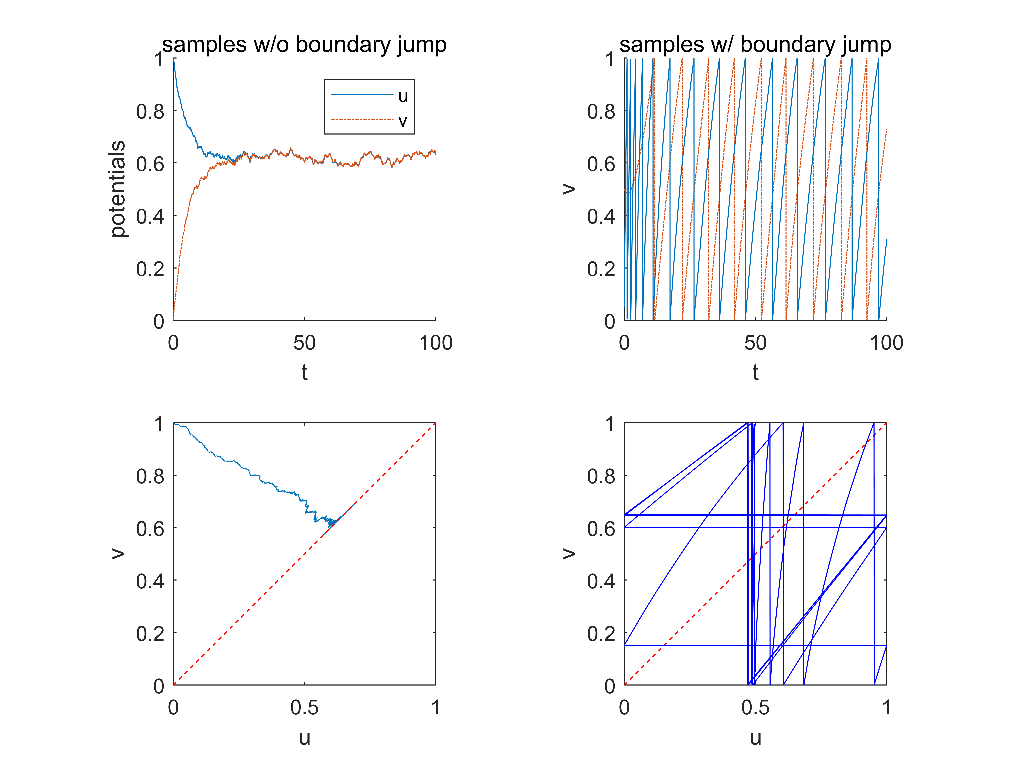
\includegraphics[width=0.5\textwidth]{BG_conv&nonconv.pdf}
\caption{\color{Gray}Comparision between non-bound-corssing (low $I$, left column) and bound-crossing (high $I$, right column). {\bf Left column.} When both $u,v$ never cross the bound $V_T=1$, $V_{0,1}$, $\epsilon(t) = u-v$ soon converges to 0, i.e. the trajectory goes to the diagonal $u=v$ on the $u-v$ plane. {\bf Right column.} However, when both samples keep firing (corssing bound and jumping back to 0), we can easily design non-converging $\epsilon$. See upper-right,  $I_{u,v}$ have different initial conditions, but reciving the same input, thus both ultimately converge to the same constant level. But constant $I_{u,v}$ make both $u,v$ periodic functions with same period but different phases, thus the error $\epsilon(t) = u-v$ never converge, i.e., the trajectory never goes to the diagonal $u=v$, but travels periodicly on the $u-v$ plane (lower-right).}
\label{BG_conv&nonconv} % \label works only AFTER \caption within figure environment
\end{figure}
\indent

\subsection{Multilevel Monte Carlo Methods}
\indent To apply MLMC reasonably, we need $\lim_{n\to \infty}|u_{\Delta t}(n)-v_{\Delta t}(n)|\to 0$ to ensure stochastic error can be canceled by large amount of samples in the same time-grid level. On the other hand, we also need $$\lim_{n\to \infty, \Delta t\to 0}|u_{\Delta t}(n)-v_{\frac{\Delta t}{2}}(2n)|\to 0$$ s.t. we can use different level simulations to cancel systematic error for the same sample.
\end{multicols}
\newpage

\begin{figure*}%s state preferences regarding figure placement here

% use to correct figure counter if necessary
%\renewcommand{\thefigure}{2}

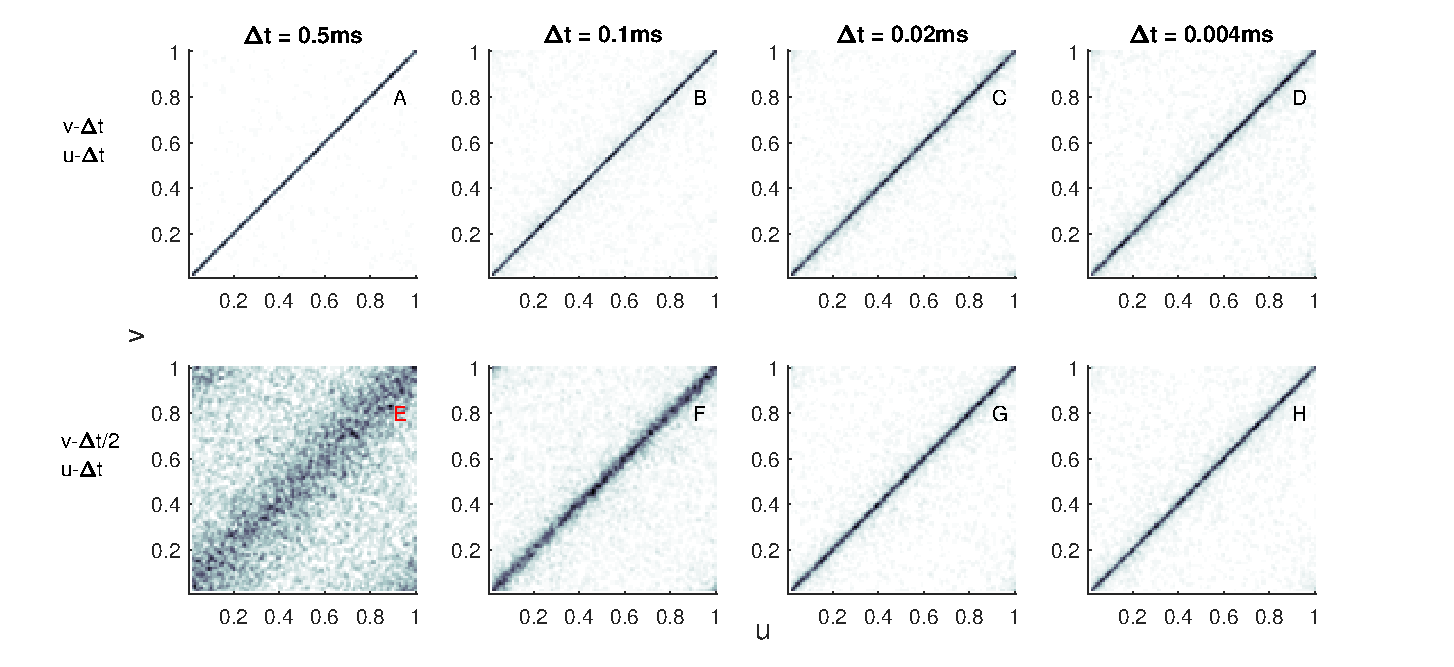
\includegraphics[width=\textwidth]{u-v.pdf}
\caption{\color{Gray} Probability density distributions for coupling $(u,v)$. For each case, we evolve 10,000 samples that initially uniformly distributed on the plane $\mathbb{T}^2=[0,1)\times[0,1)$ for 900ms with different $\Delta t$ time grids. Thus, each panel can be regarded as a numerical approximation for $\rho(u,v,t=900)$ in \ref{simpleFP} evolved from $\rho(u,v,0)\equiv 1$. For {\bf A-D}, the corresponding $u,v$s are evovled by the same time grids for "$\Delta t-\Delta t$" couplings, where $\Delta t_{u,v} = 0.5,0.1,0.02,0.004$ms, while $u,v$ using different time grids in {\bf E-H} for "$\Delta t-\Delta t/2$" couplings, where $\Delta t_{u} = 0.5,0.1,0.02,0.004$ and $\Delta t_{v} = 0.5/2,0.1/2,0.02/2,0.004/2$. For "$\Delta t-\Delta t/2$" couplings, $\rho$ more and more accumulates around diagonal when $\Delta t\to0$, while for "$\Delta t-\Delta t$" couplings larger $\Delta t$ provides better accumulations. However, when comparing {\bf D} and {\bf H}, $\rho_{0.004}^{0.004}$ and $\rho_{0.004}^{0.002}$ are pretty similar, implying that for all couplings, $\Delta t_{u,v}\to 0\Rightarrow\rho_{\Delta t_u}^{\Delta t_v}\to\rho$, regardless the relation between $\Delta t_{u,v}$.}
\label{V0_V1} % \label works only AFTER \caption within figure environment
\end{figure*}

\begin{multicols}{2}
\section{Coupling Single Neurons}
Coupling $(u,v)$ for single neurons is the simplest case, and is the base of couplings for more complex neural network. To inverstigate the coupling time and convergent rate, we consider a Fokker-Planck equation for the joint distribution $\rho(u,v,t)$. Assuming $u,v$ satisfies \ref{uIF} and \ref{vIF}, the corresponding Fokker-Planck equation should be (see details in Appendix): 
\begin{subequations}
\begin{align}
\partial_t\rho =& \partial_{u}[(g_Lu-I)\rho+\frac{f^2\nu}{2}(\partial_{u}+\partial_{v})\rho]  \nonumber\\
                       &+ \partial_{v}[(g_Lv-I)\rho+\frac{f^2\nu}{2}(\partial_{u}+\partial_{v})\rho] \nonumber\\
                      =& \partial_{u}[(g_Lu-I)\rho]+ \partial_{v}[(g_Lv-I)\rho]+\frac{f^2\nu}{2}(\partial_{u}+\partial_{v})^2\rho \label{simpleFP}
\end{align}
\end{subequations}
\indent
According to\ref{simpleFP}, there are advections of probability on both $u,v-$directions. The diffusion term, however, is only on the diagonal $u=v$. We guess $$\lim_{t\to\infty}\rho(u,v,t) = \delta(u-v),$$which leads to convergence with probvability 1. A rigorous proof for continuous $t$ turns out to be difficult, but what we really care for is numerical convergence. Consider 2 diffrent kinds of couplings for discrete time and their corresponding joint distributions $\rho_{\Delta t_u}^{\Delta t_v}$: a) When $(u,v)$ are evolved by the same time grid, i.e. $\Delta t_u=\Delta t_v$, we should have $\lim_{t\to\infty}\rho_{\Delta t}^{\Delta t}(u,v,t)= \delta(u-v)$; b) When $(u,v)$ are evolved by different time grids, such as $\Delta t_u=2\Delta t_v$, we should also have $\lim_{t\to\infty}\rho_{\Delta t}^{\Delta t/2}(u,v,t)= \delta(u-v)$. See Fig. \ref{V0_V1} for a time section when $t$ is relatively large.



\section{Coupling Neural Network}
\noindent
We still need an error estimator for spikes as it is the jump of membrane voltage making the whole dynamics highly nonlinear and does not fit the classical numerical theory for simulation. Before we get started, let's keep one important fact in mind:
\paragraph{Proposition 1} The the numerical simulation to a neuron network system, no matter how sophisticatedly connected, does obey the classical numerical convergence, as long as none of the $V_j$s hit the threshold, with the error  $O(\Delta t)$ when we use forward Euler method. 
\begin{figure}[H] %s state preferences regarding figure placement here
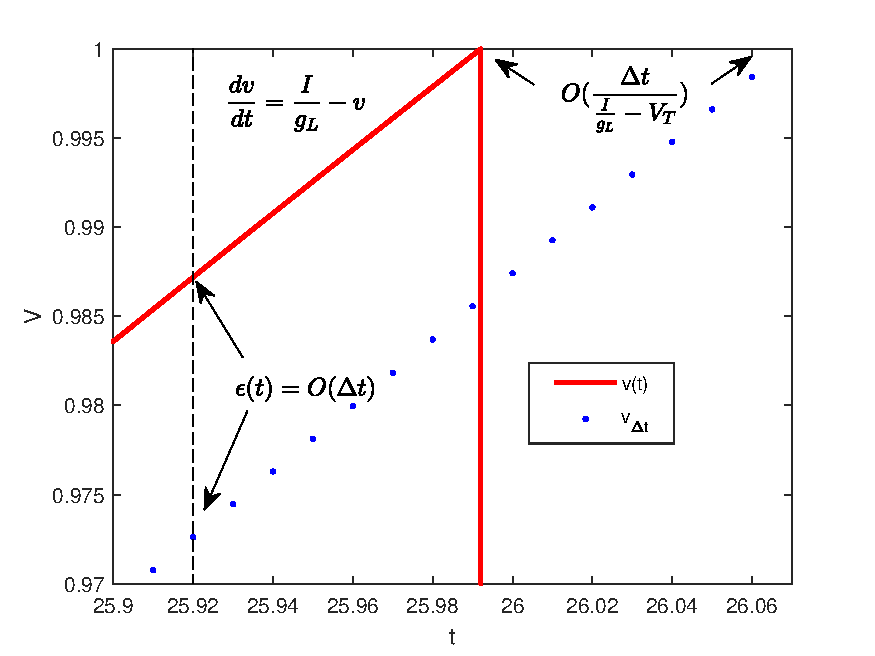
\includegraphics[width=0.5\textwidth]{t_error.pdf}
\caption{\color{Gray}"Real" solution $V(t)$ (of course it's also an mumerical solution but with much finer grids) and numerical solution $V(n\Delta t)$. We can choose the time steps much smaller that the frequency of input Possion process $\lambda$, and the decay speed of $I$ which is $\sigma_{E,I}$, thus $I$ is approximately a constant and the trajectories for $V(t)$ and $V(n\Delta t)$ can be regareded as straight lines with slope to be $I/g_L-V_{th}$.}

\label{t_error} % \label works only AFTER \caption within figure environment
\end{figure}
\indent
First, we study the spikes from only one neuron. As illustrated in Fig.\ref{t_error}, let's consider the actual solution $V(t)$ to \ref{hom-IF} and numerical solution $V_{\Delta t}(n)$ to \ref{num-hom-IF}. Before any firing event, we have $|V(n\Delta t)-V_{\Delta t}(n)|=O(\Delta t)$, and the error converge to zero in probability when $t\rightarrow\infty$. Thus, it's safe to say $|V(n\Delta t)-V_{\Delta t}(n)|=O(\Delta t)$ in the whole time period we simulate. If there is a firing event after time point $n\Delta t$, $V(n\Delta t)$ should be very close to 1 and so is $V_{\Delta t}(n)$. Also, the variation of $I$ is bounded by $O(\Delta t)$ in a small period of $\Delta t$. That's to say, the difference between he real spiketime $t_s$ and the numerical spiketime $t_{ns}$ is $O(\Delta t/(\frac{I}{g_L}-V_{th}))$, as both trajectories can be approximately regarded as straight lines before the firing event.  Now we have another important fact: 
\paragraph{Proposition 2} The time errors for spike series produced by one neuron are $O(\Delta t/(\frac{I}{g_L}-V_{th}))$, thus of magnitude $O(\Delta t)$ as long as $\frac{I}{g_L}-V_{th}$ has a lower bound, which is necessary for a neuron to fire.  \\

\indent
Now let's consider an application of Proposition 2 to a 2-neuron feed-forward case. We input Possion-like series and constant inhibitory current, for the sake of increasing the variation of $I^1$, to neuron 1. Excitory neuron 1 produce spikes as the only input to neuron 2. Proposition 1 gives us that the spiking time errors for neuron 1 is $O\Delta t$ as the numerical results for $I^1$ and $V^1$ are both $O\Delta t$ accurate, which means $I^2$ is $O\Delta t$ accurate except for several narrow time bins brought by some spikes with larger time errors. That's to say, $V^2$ and spiking series time for neuron 2 are also $O\Delta t$ accurate in general.  The details for the system is illustrated in Figure 5. \\

\indent
Therefore, {\bf{Proposition 2}} can be easily extended to \emph{all feed-forward networks} by induction, and the simulation would be trival. To convince our reader, we now simulate a feed-forward network, but with a more biological setup, i.e., each neuron is driven by a conductance-based I-F equation:
%\begin{wrapfigure}[0]{h}{\textwidth} % wrap figure should link with provious text with no \\ !!!
% the number in [] of wrapfigure is optional and gives the number of text lines that should be wrapped around the text. Adjust according to your figures height
\end{multicols}
\begin{figure*}
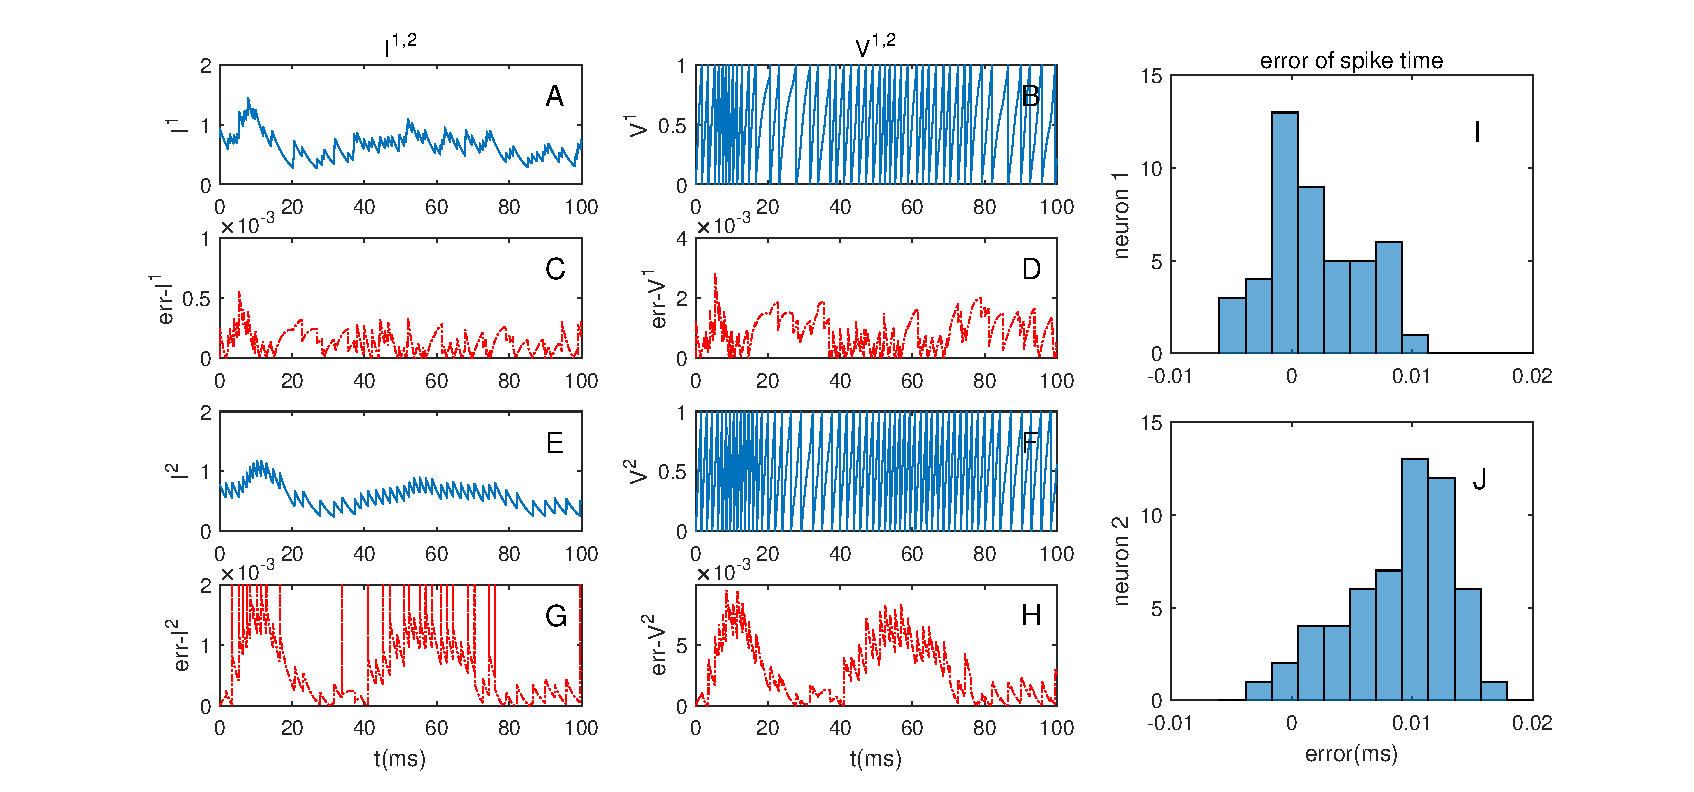
\includegraphics[width=\textwidth]{2neurons.pdf}
\caption{\color{Gray}This figure describes the numerical simulations for a 2-neuron network by $\Delta t =0.01$ms time grids. Blue curves (\textbf{A,B,E,F}) stand for the numerical results of $I^{1,2}$ and $V^{1,2}$ with $10^{-2}$ms time grid, whereas (\textbf{C,D,G,H}) red curves represent errors (given by the difference between these results with the numerical results by much finer grids) for corrsponding variables. Sub-figures in the upper half describe variables for neuron 1 (\textbf{A,B,C,D,I}), while the lower half for neuron 2 (\textbf{E,F,G,H,J}). From \textbf{C,D,I} we can see that, the errors for $I^{1}$,  $V^{1}$ and spiking series $t_{\mu^1}$ are all bounded by $O(\Delta t)$, which is no surprise from {\bf{Proposition 2}}. Thus, as $I^{2}=\sum_{\mu^1}fe^{-(t-t_{\mu^1})/\sigma}$ is a linear cimbination of a series of exponential decay functions, the error of $I^{2}$ (\textbf{G}) is made up by the “spike errors” from $t_{\mu^1}$ and calculation errors introduced when we integrate $I^{2}$. As $V^{2}$ is also integrated from $I^{2}$, we can see that the error for $V^{2}$ (\textbf{H}) is also bounded by $O(\Delta t)$, thus the same for spiking time points as $t_{\mu^2}$ (\textbf{J}).} 
\label{2neurons} % use \ref{fig1} to reference to this figure
\end{figure*}
%\end{wrapfigure} % avoid blank space here
\begin{multicols}{2}

% newpage forces a page break if you want to clearly separate materials from results
  \begin{eqnarray} 
    \frac{\mbox{d}V}{\mbox{d}t} &=&  - g_LV-G^{E}(V-V^E)-G^I(V-V^I), \nonumber\\
    \sigma_E\frac{\mbox{d}G^{E}}{\mbox{d}t} &=& -G^E+\sum_{\mu^{E}}f^{E}\delta(t-t_{\mu^{E}}),  \nonumber\\ \label{G-IF}
    \sigma_I\frac{\mbox{d}G^I}{\mbox{d}t} &=& -G^I+\sum_{\mu^I}f^I\delta(t-t_{\mu^I}). 
  \end{eqnarray}

\indent
Note that the the role $I$ plays in current-based model is now substituted by $G^E$, which receives input spikes and drives a neuron to fire.  The convergence theorm for \ref{G-IF} shouldn't be  dramatically different from \textbf{Theorm 1}, as $\frac{G^{E}(V-V^E)}{I^E}$ is bounded. We show the numerical results for a conductance-based feed-forward network with different grids in Figure. \ref{G_based_feedforward}, from which we can see {\bf{Proposition 2}} also holds, even if we change current-based model to conductance-based.
\end{multicols}
%\begin{wrapfigure}[0]{t}{\textwidth} % wrap figure should link with provious text with no \\ !!!
% the number in [] of wrapfigure is optional and gives the number of text lines that should be wrapped around the text. Adjust according to your figures height
\begin{figure*}
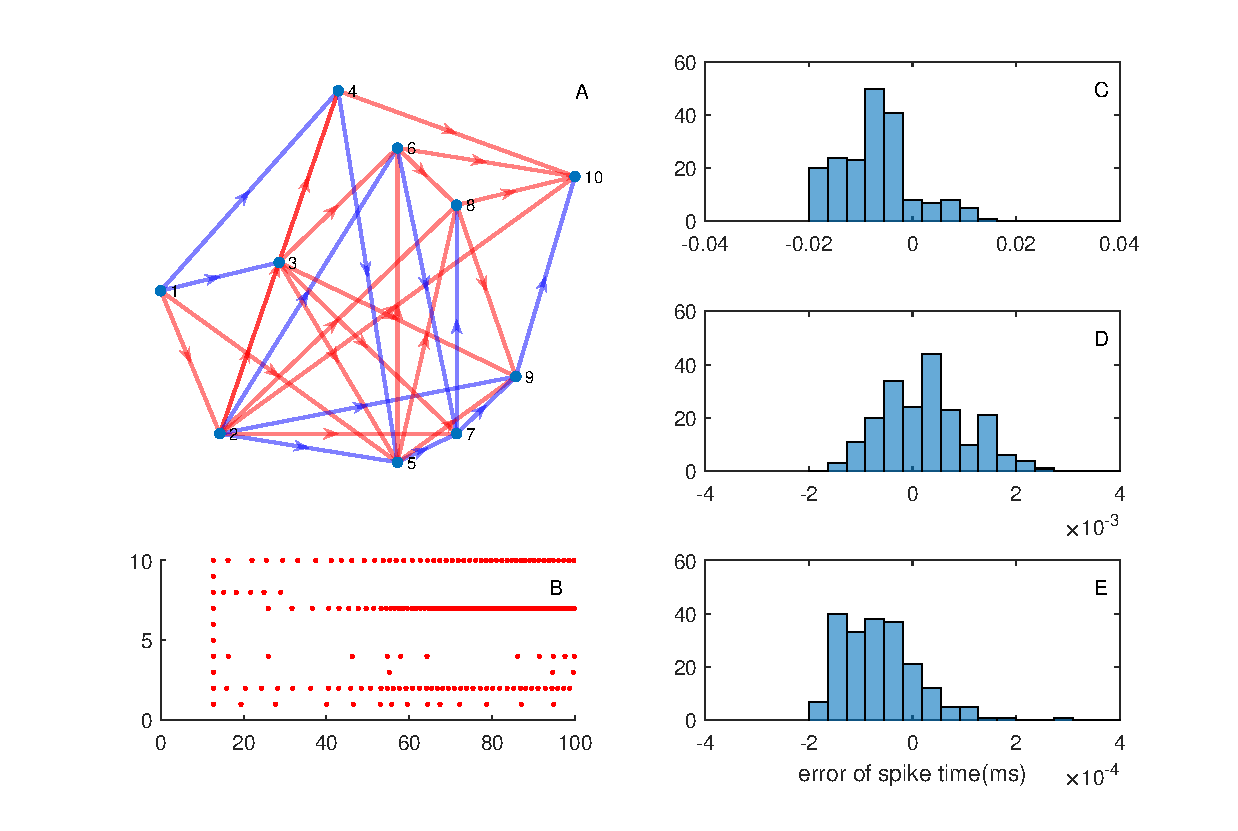
\includegraphics[width=\textwidth]{G_based_feedforward.pdf}
\caption{\color{Gray}We use the same Possion-like input to simulate a 10-neuron feed-forward neural network with 4 different grids ($\Delta t = 10^{-2},10^{-3},10^{-4} and 10^{-5}$ms). \textbf{(A)}, the topological graph for a 10-neuron feed-forward neural network, where red arrows represent excitory connections and blue arrows for inhibitory connections.  One can see from the graph that this is a network without any feedback loop. \textbf{(B)}, each read dot stands for a firing event for corresponding neuron in this network. \textbf{(C, D, E)}, we  spike time differences between $10^{-m}$ and $10^{-m-1}$ grids for the whole network, where $m = 2,3,4$. We can see the numerical results for different numerical grids do converge when grids become finer and finer.} 
\label{G_based_feedforward} % use \ref{fig1} to reference to this figure
\end{figure*}
%\end{wrapfigure} % avoid blank space here
\begin{multicols}{2}
%\begin{figure}[t] %s state preferences regarding figure placement here
%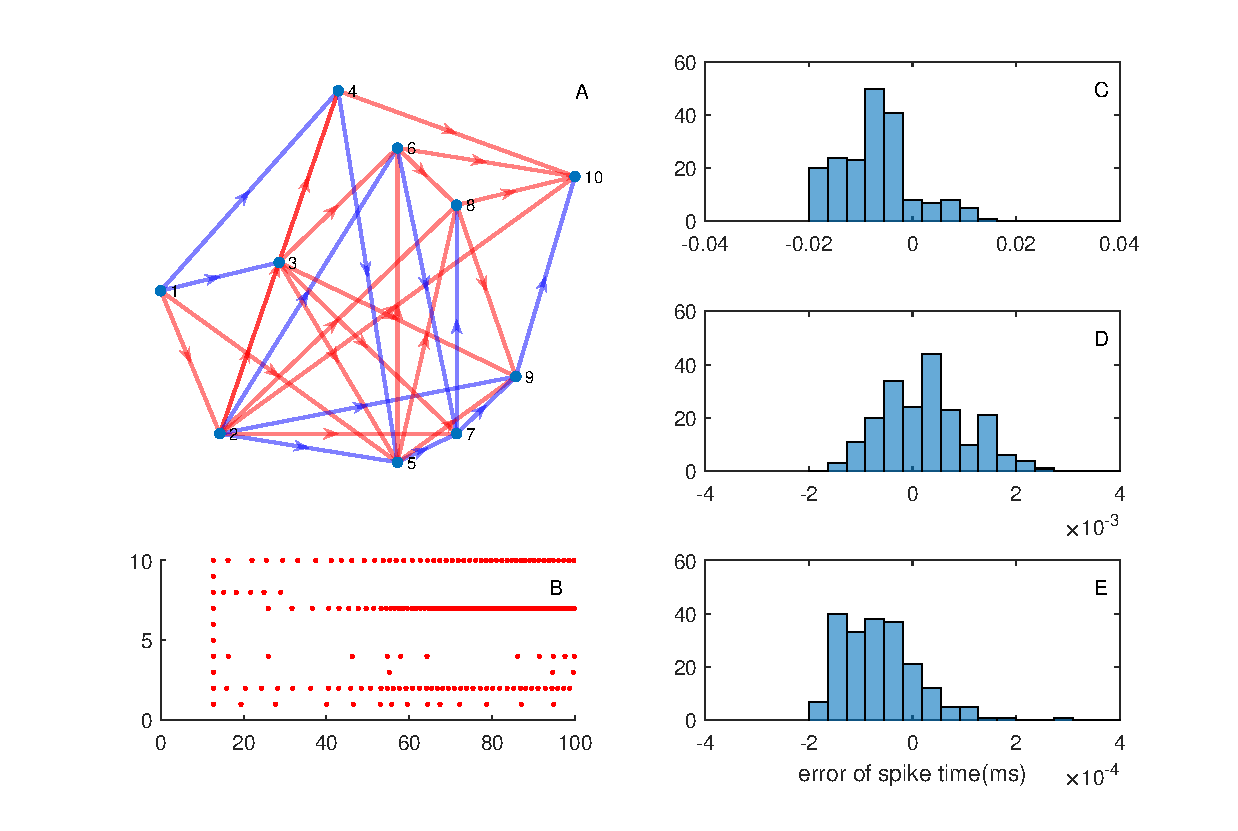
\includegraphics[width=\textwidth]{G_based_feedforward.png}
%\caption{\color{Gray} We use the same Possion-like input to simulate a 10-neuron feed-forward neural network with 4 different grids ($\Delta t = 10^{-2},10^{-3},10^{-4} and 10^{-5}$ms). %\textbf{(A)}, the topological graph for a 10-neuron feed-forward neural network, where red arrows represent excitory connections and blue arrows for inhibitory connections.  One can see from the %graph that this is a network without any feedback loop. \textbf{(B, C, D)}, we  spike time differences between $10^{-m}$ and $10^{-m-1}$ grids for the whole network, where $m = 2,3,4$. We can see %the numerical results for different numerical grids do converge when grids become finer and finer.}

%\label{G_based_feedforward} % \label works only AFTER \caption within figure environment
%\end{figure}
\newpage

\end{multicols}
\begin{figure*}[t] %s state preferences regarding figure placement here
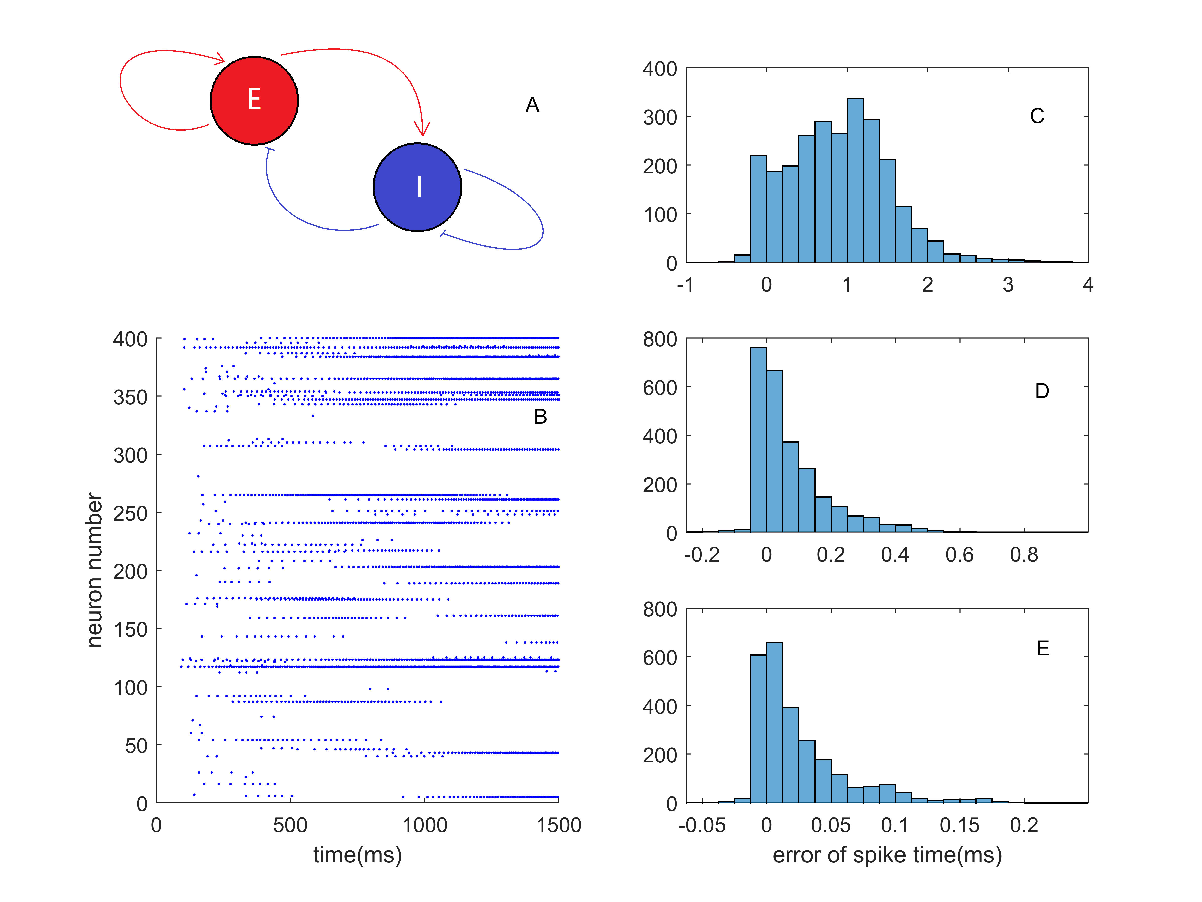
\includegraphics[width=\textwidth]{G_based_recurrent.pdf}
\caption{\color{Gray} We use the different Possion-like inputs each neuron to simulate a 400-neuron V1 network with 4 different grids ($\Delta t = 0.1,0.1*4^{-1},0.1*4^{-2}$ and $0.1*4^{-3}$ms)}.

\label{G_based_recurrent} % \label works only AFTER \caption within figure environment
\end{figure*}
\begin{multicols}{2}
So far we have investigated convergence for feed-forward networks for current based and conductance based, which is a large category of neural network. However, a biologically-realistic neural network usually consists of rich recurrent, i.e., feed-back connections. We now move to a 1024-neuron case with recurrent, which is broadly used in V1 model. One can see that the convergence still holds. However, comparing with feed-forward cases, the variance of error is much larger. This is because the MC method only works when the neurons firing patern is homogenized, i.e, with weak correlation. If we consider an extreme case, that several connected neurons firing together, which are synchronized, it's clear that no numerical method can control the error when $\Delta t \rightarrow 0$.

\section*{Discussion}



\section*{Acknowledgments}
We thank just about everybody.

\section*{Appendix}
To restrict our discussion to $(2+1)$ dimentional PDE (or numerical PDE), we write the F-P eqns for a homogenized version of \ref{1IF}, and it's numerical form:
  \begin{eqnarray} 
\label{hom-IF}
    \frac{\mbox{d}V_{0,1}}{\mbox{d}t} &=&  - g_LV_{0,1}+\sum_{\mu}f\delta(t-t_{\mu}),      
     \\
\label{num-hom-IF}
   \frac{V^{(n+1)h}_{0,1}-V^{nh}_{0,1}}{h} &=& - g_LV^{nh}_{0,1}+\sum_{nh\leq\mu<(n+1)h}f\delta(t-t_{\mu}).
  \end{eqnarray} 
where $V_1(0) - V_0(0)= \epsilon$ is satisfied for both \ref{hom-IF} and \ref{num-hom-IF}. Inspired by {\bf{$I_1$}}, we now look at probability distribution $\rho(V_0,V_1,t)$ on time $t$ (for continuous or discrete time) and plane $V_0\times V_1$. \\
\indent
For \ref{hom-IF}, the F-P eqn is
  \begin{eqnarray}
\label{hom-FP}
\partial_t\rho(V_0,V_1,t) &=& \partial_{V_0}(g_LV_0\rho)+\partial_{V_1}(g_LV_1\rho)+\lambda[\rho(V_0-f,V_1-f,t)-\rho(V_0,V_1,t)].
  \end{eqnarray} 
For small $f$, with Taylor expansion we could rewrite \ref{hom-IF} into 
  \begin{eqnarray}
\partial_t\rho &=& \partial_{V_0}(g_LV_0\rho)+\partial_{V_1}(g_LV_1\rho)+\lambda[-f(\partial_{V_0}+\partial_{V_1})\rho+\frac{f^2}{2}(\partial_{V_0}+\partial_{V_1})^2\rho].  \nonumber\\
\label{hom-con-FP}
               &=& \partial_{V_0}[(g_LV_0-f\lambda)\rho+\frac{f^2\lambda}{2}(\partial_{V_0}+\partial_{V_1})\rho] + \partial_{V_1}[(g_LV_1-f\lambda)\rho+\frac{f^2\lambda}{2}(\partial_{V_0}+\partial_{V_1})\rho],
  \end{eqnarray}
where we often use $\mu$ to substitute $f\lambda$ and $\sigma^2$ for $f^2\lambda$. According to the equation of continuity $\partial_t\rho+\partial_{V_0}J_{V_0}+\partial_{V_1}J_{V_1}=0$, we have:
  \begin{eqnarray}
J_{V_0} &=& -(g_LV_0-\mu)\rho-\frac{\sigma^2}{2}(\partial_{V_0}+\partial_{V_1})\rho,  \nonumber\\
\label{fluxs}
J_{V_1} &=& -(g_LV_1-\mu)\rho-\frac{\sigma^2}{2}(\partial_{V_0}+\partial_{V_1})\rho,
  \end{eqnarray}
with natural boundary conditions (similar to (4.25) in \cite{FPTaoCai}):
  \begin{eqnarray}
J_{V_0}(0,v_1,t) &=& J_{V_0}(1,v_1,t), \quad \rho(0,v_1,t) =  \rho(1,v_1,t) \nonumber\\
\label{B.C.}
J_{V_1}(v_0,0,t) &=& J_{V_1}(v_0,1,t), \quad \rho(v_0,0,t) =  \rho(v_0,1,t).
  \end{eqnarray}
\indent
For \ref{num-hom-IF}, we consider the condition probability for $\rho(V_0,V_1,t+\Delta t)$ giving conditions for $V_0(t),V_1(t)$. Assuming $\Delta t$ is too small for more than 1 input events occur in $[t,t+\Delta t)$, then there are only 2 choices for the system in this time period: receiving one input spike with probability $\lambda\Delta t$, and receiving nothing with probability $1-\lambda\Delta t$. Thus, we have:
  \begin{eqnarray}
&&\mathbb{E}[\delta(v-V_0(t+\Delta t))\delta(v-V_1(t+\Delta t))|V_0(t),V_1(t)] \nonumber\\
 &=& \lambda\Delta t \delta(v-V_0(t)-f)\delta(v-V_1(t)-f) \nonumber\\
\label{Exp}
&+&(1-\lambda\Delta t) \delta(v-V_0(t)+g_LV_0(t)\Delta t)\delta(v-V_1(t)+g_LV_1(t)\Delta t).
\end{eqnarray}
Using Taylor expansion for $\delta$-function:
$$
\delta(v-V_i(t)+g_LV_i(t)\Delta t) = \delta(v-V_i(t))+\partial_v[\delta(v-V_i(t))g_LV_i(t)]\Delta t + O(\Delta^2 t),
$$
we can rewrite \ref{Exp} into probability form:
\begin{eqnarray}
\label{num-hom-FP}
\rho_{\Delta t}(V_0,V_1,t+\Delta t) &=& \lambda\Delta t\rho_{\Delta t}\Delta t(V_0-f,V_1-f,t) \nonumber\\
&+& (1-\lambda\Delta t)[\rho_{\Delta t}+\partial_{V_0}(g_LV_0\rho_{\Delta t})\Delta t+\partial_{V_1}(g_LV_1\rho_{\Delta t})\Delta t]+O(\Delta^2 t),  
\end{eqnarray}
where $\rho_{\Delta t}$ is the probability distribution function for discrete-time Fokker-Planck equation in \ref{num-hom-FP}. One can easily check that \ref{num-hom-FP} is consistent with \ref{hom-FP} at order $O(\Delta t)$, thus the "numerical" solution converges to the "actual" solution for  \ref{hom-FP} when $\Delta t \rightarrow 0$. Thus, the globle error for $\Delta t-\Delta t$ grid converge to the globle error for actual solution in probability.\\
\indent
To use numerical results from different grids, we also need to consider the case that $V_0$ is evloved by $\Delta t$-grids and $V_1$ is evolved by $\frac{\Delta t}{2}$-grids, or $\Delta t-\frac{\Delta t}{2}$ grids, to see if the globle error $V_0-V_1$ diminish in time. Similar to \ref{Exp}, we could write the conditional expectation as:
  \begin{eqnarray}
&&\mathbb{E}[\delta(v-V_0(t+\Delta t))\delta(v-V_1(t+\Delta t))|V_0(t),V_1(t)] \nonumber\\
 &=& \frac{\lambda\Delta t}{2} \delta[v-V_0(t)-f]\delta[v-V_1(t)-f+g_L(V_1(t)+f)\frac{\Delta t}{2}] \nonumber\\
 &+& \frac{\lambda\Delta t}{2} \delta[v-V_0(t)-f]\delta[v-V_1(t)-f+g_LV_1(t)\frac{\Delta t}{2}] \nonumber\\
\label{Exp2}
&+&(1-\lambda\Delta t) \delta[v-V_0(t)+g_LV_0(t)\Delta t]\delta[v-V_1(t)+g_LV_1(t)\frac{\Delta t}{2}+g_LV_1(t)(1-g_L\frac{\Delta t}{2})\frac{\Delta t}{2}].
\end{eqnarray}

Using Taylor expansion for $\delta$-function, we know the corresponding F-P eqn is exactly the same as \ref{num-hom-FP} if we discard terms with order higher than $O(\Delta t)$. This is suggested by Fig.\ref{V0_V1}, as if we fix a finite time point $t$ both 2 series of discrete-time distributions ($\Delta t-\Delta t$ and $\Delta t-\frac{\Delta t}{2}$) seem to have the same limit when $\Delta t\rightarrow 0$, i.e., $\rho_{\Delta t}(V_0,V_1,t)\rightarrow \rho(V_0,V_1,t)$. Also, it is implied by the figure that the density for $\rho(V_0,V_1,t)$ should aggregate along the diagonal $V_0=V_1$ when $t\rightarrow \infty$.\\
\indent
We have proved that both $\Delta t-\Delta t$ and $\Delta t-\frac{\Delta t}{2}$ grids yield discrete-time F-P eqns that are consistant with \ref{hom-FP}. The solutions to them thus converge to \ref{hom-con-FP} when $f\rightarrow 0$. The last part of proof for convergence in probability is to show that the solution to \ref{hom-con-FP} converge to the diagonal $V_0=V_1$ when $t\rightarrow\infty$.


\subsection*{Steady Solution on the Diagonal}
We now start to show that the steady distribution $\rho_{\infty}(V_0,V_1)$ can only be non-zero on the diagonal $V_0=V_1$. Before that, we need several lemmas for preparation. 

\paragraph{Lemma 1} For the steady solution $p_{\infty}(v)$ of the F-P eqn for only 1 neuron:
\begin{eqnarray}
\label{FP1}
\partial_tp(v,t) &=&\partial_v\left\{ [g_Lv-\mu]p+\frac{\sigma^2}{2}\partial_vp \right\}, \\
m(t)&=&J(V_T,t)= -[g_Lv-\mu]p-\frac{\sigma^2}{2}\partial_vp, \quad p(0,t)=p(1,t).
\end{eqnarray}
we have $M_1=\mu-m/g_L$ and $M_2=\mu M_1+[\sigma^2(1-p_{\infty}(1))-m]/(2g_L)$ for $M_1$ and $M_2$ are the first 2 order moments of $p_{\infty}(v)$. \\
{\bf{Proof.}} 
\begin{eqnarray}
\frac{\mbox{d}M_j}{\mbox{d}t}&=&\int_0^1{v^j\partial_tp(v,t)\mbox{d}t} \nonumber\\
            &=&\int_0^1{v^j\partial_v\left\{ [g_Lv-\mu]p+\frac{\sigma^2}{2}\partial_vp \right\}\mbox{d}t} \nonumber\\
            &=& -m-j[g_LM_j-g_L\mu M_{j-1}+\frac{\sigma^2}{2}(V_T^{j-1}p(1,t)-V_r^{j-1}p(0,t)-(j-1)M_{j-2})]. \nonumber
\end{eqnarray}
\indent Especially, for $j=1,2$, as $M_0=\int_0^1{p(v,t)\mbox{d}t}=1$, we have:
\begin{eqnarray}
\frac{\mbox{d}M_1}{\mbox{d}t} &=& -m-g_L(M_1-\mu), \nonumber\\
\frac{\mbox{d}M_2}{\mbox{d}t} &=& -m-2[g_LM_2-g_L\mu M_1+\frac{\sigma^2}{2}(p(1,t)-1)]. \nonumber
\end{eqnarray}
So we could find the steady states for $M_1$ and $M_2$.

\paragraph{Lemma 2} Consider $\mathbb{E}(V_0V_1)$ for $\rho_{\infty}(V_0,V_1)$, we have 
\begin{eqnarray}
\label{L2}
\mathbb{E}(V_0V_1) = \mu^2-\frac{\mu m}{g_L}+\frac{\sigma^2(1-p_{\infty}(1))}{2g_L}-\frac{1}{g_L}\int_0^1{m(V)V\mbox{d}V}.
\end{eqnarray}
{\bf{Proof.}} 
\begin{eqnarray}
\frac{\mbox{d}\mathbb{E}(V_0V_1)}{\mbox{d}t} 
&=& \int_0^1{\int_0^1{V_0V_1\partial_t\rho\mbox{d}V_0}\mbox{d}V_1} \nonumber\\
&=& -\int_0^1{V_0\mbox{d}V_0\int_0^1{V_1\mbox{d}J_{V_1}}}-\int_0^1{V_1\mbox{d}V_1\int_0^1{V_0\mbox{d}J_{V_0}}}.
\end{eqnarray}
\indent
As $V_0$ and $V_1$ are commutable in \ref{hom-con-FP}, i.e., they have the same status, the stationary distribution function $\rho_{\infty}(V_0,V_1)$ should be a symmetrical function along the diagonal $V_0=V_1$, thus $\int_0^1{V_0\mbox{d}V_0\int_0^1{V_1\mbox{d}J_{V_1}}}=\int_0^1{V_1\mbox{d}V_1\int_0^1{V_0\mbox{d}J_{V_0}}}$, giving us that
\begin{eqnarray}
\frac{\mbox{d}\mathbb{E}(V_0V_1)}{\mbox{d}t}=0 
&\implies& \int_0^1{V_1\mbox{d}V_1\int_0^1{V_0\mbox{d}J_{V_0}}}=0 \nonumber\\
&\implies& \int_0^1{V_1\mbox{d}V_1 \left\{ -m(V_1) - \int_0^1{[(g_LV_0-\mu)\rho+\frac{\sigma^2}{2}(\partial_{V_0}+\partial_{V_1})\rho]\mbox{d}V_0}  \right\}}=0 \nonumber\\
&\implies& -\int_0^1{m(V_1)V_1\mbox{d}V_1}-g_L\mathbb{E}(V_0V_1)+\mu M_1-\frac{\sigma^2}{2}(p_{\infty}(1)-1)=0
\end{eqnarray}
With {\bf{Lemma 1}}, we know that \ref{L2} is true.

\paragraph{Lemma 3} $\rho_{\infty}$ attaches 0 on the boundary, except the 4 corners.\\
{\bf{Proof.}}\\
\indent
Again, as $V_0$ and $V_1$ are commutable in \ref{hom-con-FP}, we know that $\rho_{\infty}(V_0,V_1)=\rho_{\infty}(V_1,V_0)$. So
\begin{eqnarray}
\partial_{V_0}J_{V_0} + \partial_{V_1}J_{V_1}= 0 
&\implies& \partial_{V_0}J_{V_0}(x,y)+\partial_{V_0}J_{V_0}(y,x) = 0 \nonumber\\
&\implies& J_{V_0}(x,y)+J_{V_0}(y,x) = f(y). \nonumber
\end{eqnarray}
As $J_{V_0}(0,y)=J_{V_0}(1,y)$, we then have $J_{V_0}(y,0) = J_{V_0}(y,1)$ for arbitary $y\not\equiv 0,1$. Thus,
$$
(y-\lambda f)\rho(y,0)+(\partial_{V_0}+\partial_{V_1})\rho(y,0) = (y-\lambda f)\rho(y,1)+(\partial_{V_0}+\partial_{V_1})\rho(y,1).
$$
\indent
Combining this with the boundary condition that $\rho(y,0)=\rho(y,1)$, we can see that $\partial_{V_0}\rho(y,0) = \partial_{V_0}\rho(y,1) \implies \partial_{V_1}\rho(0,y) = \partial_{V_1}\rho(1,y)$. Use $J_{V_0}(0,y)=J_{V_0}(1,y)$ and $\rho(0,y)=\rho(1,y)$ again, now we have 
$$
(0-\lambda f)\rho(0,y)+(\partial_{V_0}+\partial_{V_1})\rho(0,y) = (1-\lambda f)\rho(1,y)+(\partial_{V_0}+\partial_{V_1})\rho(1,y).
$$
So $\rho(0,y)=0$ for arbitary $y\not\equiv 0,1$.\\
\indent
Now we can go to prove the main theorm for the steady solution.

\paragraph{Theorm 1} The steady distribution for \ref{hom-con-FP} has a support on the diagonal line $V_0 = V_1$.\\
{\bf{Proof.}}\\
From {\bf{Lemma 3}} we can see that $\int_0^1{m(V)V\mbox{d}V}=m(0)\times 0+m(1)\times 1=m/2$ as $m(0)=m(1)$. Thus combining {\bf{Lemma 1}} with {\bf{Lemma 2}} we get 
\begin{eqnarray}
\mathbb{E}(V_0V_1) 
&=& \mu^2-\frac{\mu m}{g_L}+\frac{\sigma^2(1-p_{\infty}(1))}{2g_L}-\frac{m}{2g_L} \nonumber\\
&=& M_1^2+M_2 = \mathbb{E}(V_0)\mathbb{E}(V_1)+\sqrt{\mbox{var}(V_0)\mbox{var}(V_1)},
\end{eqnarray}
which exactly means that $\mbox{cor}(V_0,V_1)=[\mathbb{E}(V_0V_1) -\mathbb{E}(V_0)\mathbb{E}(V_1)]/\sqrt{\mbox{var}(V_0)\mbox{var}(V_1)}=1$. Thus, stochastic veriables $V_0$ and $V_1$ are fully synchronized when $t\rightarrow \infty$. Convergence in propability is then proved.


\begin{thebibliography}{3}                                          
\addcontentsline{toc}{chapter}{References}
  \bibitem{Giles2008} Giles, Michael B. "Multilevel monte carlo path simulation." Operations Research 56.3 (2008): 607-617.
  \bibitem{FPTaoCai} Cai, David, et al. "Kinetic theory for neuronal network dynamics." Communications in Mathematical Sciences 4.1 (2006): 97-127.
  \bibitem{MFE} Rangan, Aaditya V, et al. "Dynamics of spiking neurons: between homogeneity and synchrony." J Comput Neurosci (2013) 34:433–460.
\end{thebibliography}

\end{multicols}
\end{document}